\chapter{Introduction to the RGB-D Visual Odometry Problem}%
\label{cha:rgbd_vo}

\minitoc%
\clearpage

\section{Image Formation (copied)}%
\label{sec:image-formation}

\alert{Copied from cremers mvg, need reformulation}

\subsection{Historic Remarks}%
\label{sub:historic_remarks}


\begin{figure}[h]
\centering
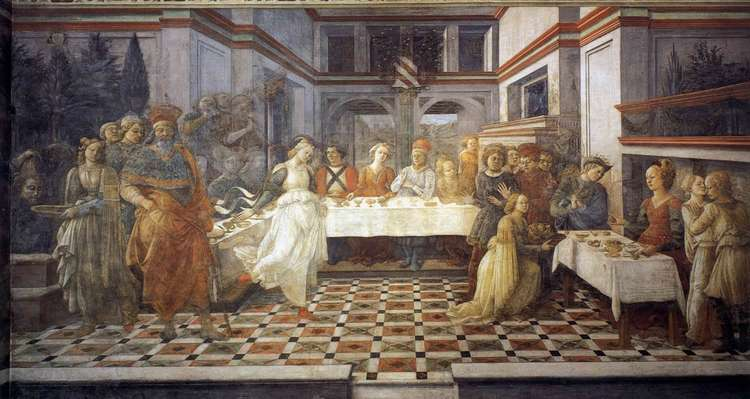
\includegraphics[width=0.5\columnwidth]{assets/img/lippi_feast_herod.jpg}
\caption{Filippo Lippi, ``The Feast of Herod: Salome's Dance.''
Fresco, Cappella Maggiore, Duomo, Prato, Italy, c.1460--1464.}%
\label{fig:lippi_feast_herod}
\end{figure}

\begin{figure}[h]
\centering
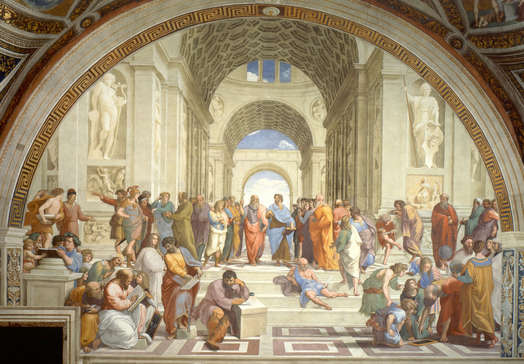
\includegraphics[width=0.5\columnwidth]{assets/img/raphael_school_athens.jpg}
\caption{Raphael, The School of Athens (1509)}%
\label{fig:raphael_school_athens}
\end{figure}

\begin{figure}[h]
\centering
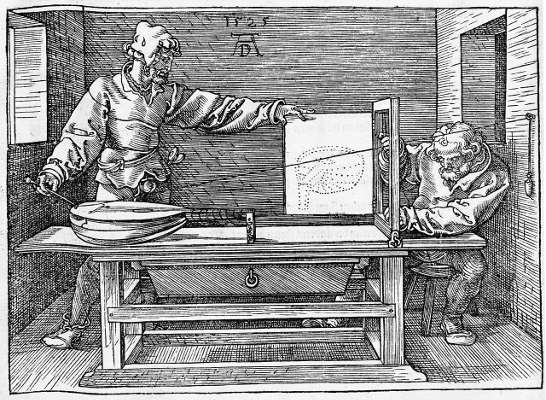
\includegraphics[width=0.5\columnwidth]{assets/img/durer_perspective_machine.jpg}
\caption{D\"urer's perspective machine (1525)}%
\label{fig:durer_perspective_machine}
\end{figure}

The study of the image formation process has a long history.
The earliest formulations of the geometry of image formation
can be traced back to \textbf{Euclid} (4th century B.C.).
Examples of a partially correct \textbf{perspective projection}
are visible in the \textbf{frescoes and mosaics of Pompeii} (1 B.C.).\\

These skills seem to have been lost with the fall of the Roman empire.
Correct perspective projection emerged again around 1000 years later
in early \textbf{Renaissance art}.\\

Among the proponents of perspective projection are the
Renaissance artists \textbf{Brunelleschi, Donatello} and \textbf{Alberti}.
The first treatise on the projection process, \textbf{``Della Pittura''},
was published by \textbf{Leon Battista Alberti}.\\

Appart from the geometry of image formation, the study of the
interaction of light with matter was propagated by artists like
\textbf{Leonardo da Vinci} in the 1500s and by Renaissance painters
such as \textbf{Caravaggio} and \textbf{Raphael}.\\

In Figure~\ref{fig:lippi_feast_herod} and Figure~\ref{fig:raphael_school_athens}
the perspective emerges from the vanishing point.

\begin{figure}[h]
\centering
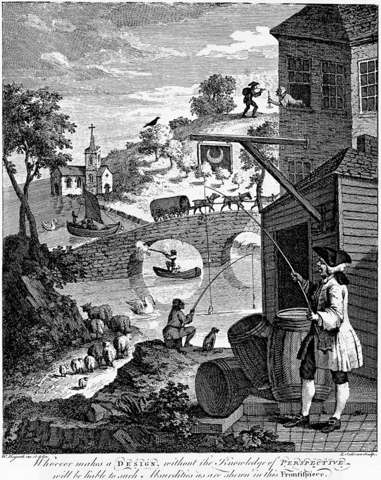
\includegraphics[width=0.5\columnwidth]{assets/img/hogarth_satire.jpg}
\caption{Satire by Hogarth 1753}%
\label{fig:hogarth_satire}
\end{figure}

\begin{figure}[h]
\centering
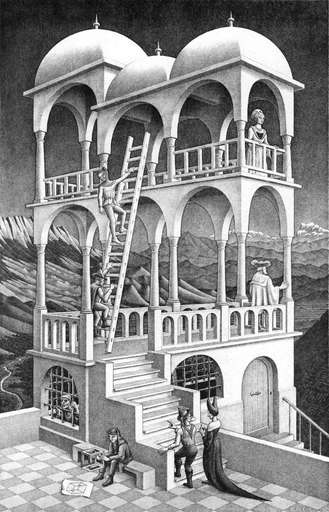
\includegraphics[width=0.5\columnwidth]{assets/img/escher_belvedere.jpg}
\caption{Escher, Belvedere 1958}%
\label{fig:escher_belvedere}
\end{figure}

D\"urer devised a machine to get a perspectively correct image,
see Figure~\ref{fig:durer_perspective_machine}.
It is a manual reproduction of what a camera does today.\\

Many artists played with those perspective rules to create images
that seems locally correct but have inconsitent depth or gravity, like
in Figures~[\ref{fig:hogarth_satire},\ref{fig:escher_belvedere}].


\subsection{Projective Geometry}%
\label{sub:projective_geometry}


In order to formally write transformations by linear operations,
we made extensive use of \textbf{homogeneous coordinates} to represent
3D point as a 4D-vector $(X,Y,Z,1)$ with the last coordinate fixed to 1.
This normalization is not always necessary. One can represent 3D points
by a general 4D vector:
\[
	\bm{X} = (XW, YW, ZW, W)\ \in\ \R^4
\]
In general, an \textbf{n-dimensional projective space} $\mathbb{P}^n$
is the set of all one-dimensional subspaces (i.e.\ lines through the origin)
of the vector space $\R^{n+1}$.
A point $p \in \mathbb{P}^n$ can then be assigned homogeneous coordinates
$\bm{X} = \tr{(x_1, \ldots, x_{n+1})}$, among which at least one $x$ is nonzero.
For any nonzero $\lambda \in \R$, the coordinates
$\bm{Y} = \tr{(\lambda x_1, \ldots, \lambda x_{n+1})}$
represent the same point $p$.


\subsection{Mathematical Representation}%
\label{sub:mathematical_representation}


\begin{figure}[h]
\centering
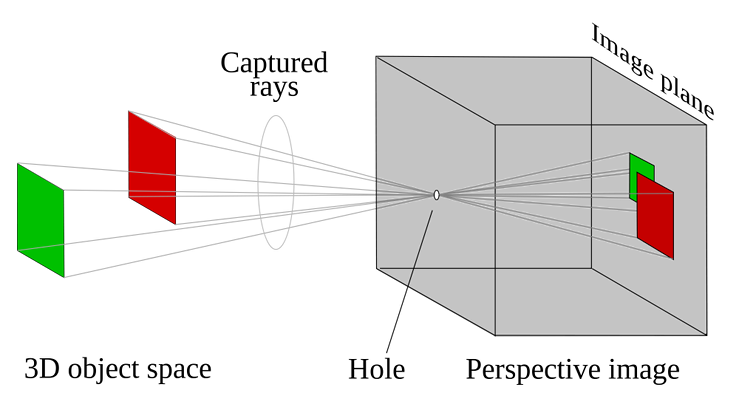
\includegraphics[width=0.5\columnwidth]{assets/img/pinhole_camera.png}
\caption{Pinhole camera model}%
\label{fig:pinhole_camera}
\end{figure}

\begin{figure}[h]
\centering
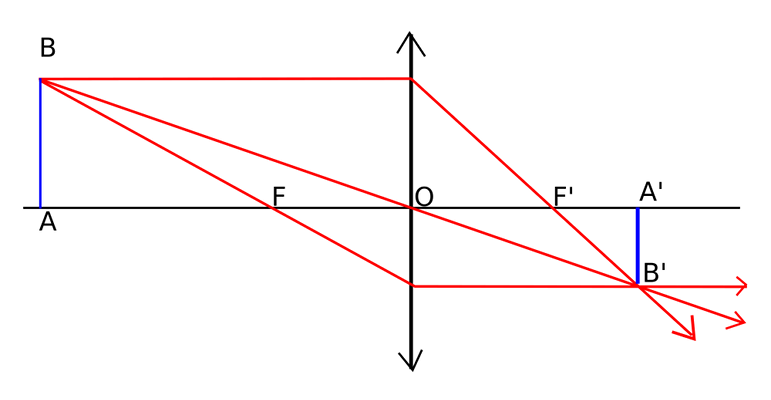
\includegraphics[width=0.5\columnwidth]{assets/img/convex_lense.png}
\caption{Thin convex lense model}%
\label{fig:convex_lense}
\end{figure}

Perspective projection emerges by the so-called pinhole camera model
(see Figure~\ref{fig:pinhole_camera}).
It's main issue is that the hole has to be very small,
perventing light to enter the capture device.
In order to augment the the amount of light we use lenses\\

As visible in (Figure~\ref{fig:convex_lense}), the image is upside down
in the image plan. In order to avoid dealing with minus signs in the
equations, we pretend that the image plan is virtually on the same
side than the object. The perspective thansformation $\pi$ is given by
\[ \pi : \R^3 \rightarrow \R^2; \quad
	\bm{X} \mapsto x = \pi(\bm{X}) =
	\begin{pmatrix}
		f \frac{X}{Z} \\
		f \frac{Y}{Z} \\
	\end{pmatrix}
\]
Where $f$ is the focal length, $X,Y,Z$ are the object coordinates
in the 3D world, the $z$ axis being the camera axis.
The one challenge we have to overcome, is that this transformation is non linear.\\

In order to do so, we will use \textbf{homogeneous coordinates},
which is basically similar to multiplying everything by $Z$:
\[ Z \bm{x} = Z \begin{pmatrix} x \\ y \\ 1 \end{pmatrix} =
	\begin{pmatrix}
		f & 0 & 0 & 0 \\
		0 & f & 0 & 0 \\
		0 & 0 & 1 & 0 \\
	\end{pmatrix}
	\begin{pmatrix}
		X \\ Y \\ Z \\ 1
	\end{pmatrix}
	= K_f \Pi_0 \bm{X}
\]
Where we have introduced the two matrices
\[K_f \equiv
	\begin{pmatrix}
		f & 0 & 0 \\
		0 & f & 0 \\
		0 & 0 & 1 \\
	\end{pmatrix}
	\quad \text{and} \quad
	\Pi_0 \equiv
	\begin{pmatrix}
		1 & 0 & 0 & 0 \\
		0 & 1 & 0 & 0 \\
		0 & 0 & 1 & 0 \\
	\end{pmatrix}
\]
The matrix $\Pi_0$ is referred to as the \textbf{standard projection matrix}.
A first order approximation can consider that all object points
are approximately at the same distance $\lambda > 0$. Thus we obtain:
\[\lambda \bm{x} = K_f \Pi_0 \bm{X}\]

We know that due to the \textbf{rigid motion of the camera},
the point $\bm{x}$ \textbf{in camera coordinates} is given as a function
of the point in \textbf{wold coordinates} $\bm{X}_0$ by:
\[\bm{X} = R \bm{X}_0 + T\]
or in homogeneous coordinates:
\[\bm{X} = g \bm{X}_0 = \begin{pmatrix}R & T \\ 0 & 1\end{pmatrix} \bm{X}_0\]
In total, the transformation from world coordinates to image coordinates
is therefore given by:
\[\boxed{\lambda\ \bm{x} = K_f\ \Pi_0\ g\ \bm{X}_0}\]


\subsection{Intrinsic Parameters}%
\label{sub:intrinsic_parameters}


If the camera is not centered at the optical center, we have an additional
translation $o_x, o_y$. The point were the optical axis intersects
the image plan is called the \textbf{principal point}.\\

If pixels do not have unit scale, we need to introduce
additional scaling factors $s_x$ and $s_y$.
If pixels are not rectangular, we also have a \textbf{skew factor} $s_{\theta}$.\\

The transformation from initial real world coordinates to final pixel coordinates
follows the following steps:
World (3D, $\bm{X}_0$) $\mapsto$ Camera (3D, $\bm{X}$)
$\mapsto$ Image (2D, $\bm{x}$) $\mapsto$ Pixel (2D, $\bm{x'}$).\\

The pixel coordinates $\bm{x'} = (x',y',1)$ are given by:
\[\lambda \begin{pmatrix}x' \\ y' \\ 1\end{pmatrix} =
	K_s\ K_f\ \Pi_0
	\begin{pmatrix}X \\ Y \\ Z \\ 1\end{pmatrix}
\]
where
\[K_s = \begin{pmatrix}
		s_x & s_{\theta} & o_x \\
		0 & s_y & o_y \\
		0 & 0 & 1 \\
	\end{pmatrix}
	\quad K_f =
	\begin{pmatrix}
		f & 0 & 0 \\
		0 & f & 0 \\
		0 & 0 & 1 \\
	\end{pmatrix}
\]
We call $K = K_s\ K_f$ the \textbf{intrinsic parameter matrix}.\\

Therefore, as a function of world coordinates, we have:
\[\boxed{ \lambda\ \bm{x'} = \Pi\ \bm{X}_0
	= K\ \Pi_0\ g\ \bm{X}_0}
\]
The $3 \times 4$ matrix $\Pi$ is called a \textbf{general projection matrix}.
If we get rid of $\lambda$ we obtain the following coordinates:
\[ x' = \frac{\tr{\pi_1} \bm{X}_0}{\tr{\pi_3} \bm{X}_0},\quad
 y' = \frac{\tr{\pi_2} \bm{X}_0}{\tr{\pi_3} \bm{X}_0},\quad
 z' = 1
\]
where $\tr{\pi_1}, \tr{\pi_2}, \tr{\pi_3} \in \R^4$
are the three rows of the projection matrix $\Pi$.


\subsection{Radial Distortion}%
\label{sub:radial_distortion}


\begin{figure}[h]
\centering
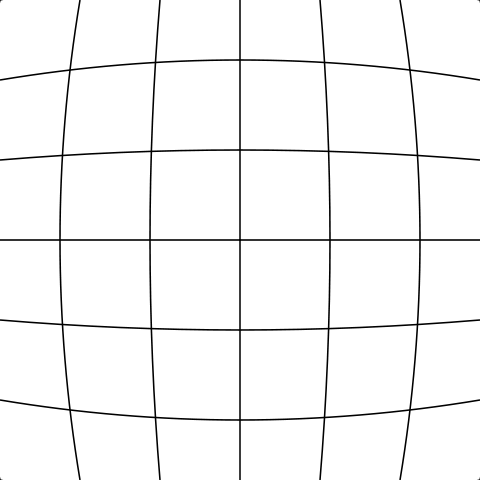
\includegraphics[width=0.5\columnwidth]{assets/img/barrel_distortion.png}
\caption{Grid projection with radial distortion.}%
\label{fig:radial_distortion}
\end{figure}

The intrinsic parameters in the matrix $K$ model linear distortions
in the transformation to pixel coordinates.
In practice however, one can also encounter significant
\textbf{distortions along the radial axis}~[\ref{fig:radial_distortion}],
in particular in a wide field of view is used or if one uses cheaper cameras
such as webcams.
A simple effective model for such distortions is:
\[
	x = x_d ( 1 + a_1 r^2 + a_2 r^4 ),
	y = y_d ( 1 + a_1 r^2 + a_2 r^4 )
\]
where $\bm{x} \equiv (x_d, y_d)$ is the distorted point,
$r^2 = \|\bm{x}\|^2$.
Usually, $a_1$ and $a_2$ are estimated through a calibration step.\\

Other more sophisticated models exist (Devernay and Faugeras '95).
Parameters are computed from
\textbf{distortions of straight lines} (see Figure~\ref{fig:radial_distortion})
or \textbf{simultaneously with the 3D reconstruction}
(Zhang '96, Stein '97, Fitzgibbon '01).

\section{Representing a Moving Scene (copied)}%
\label{sec:moving-scene}

\alert{Copied from cremers mvg, need reformulation}

\subsection{The Origins of 3D Reconstruction}%
\label{sub:the_origins_of_3d_reconstruction}

The goal to reconstruct the three-dimensional structure of the world from
a set of two-dimensional views has long history in computer vision.
It is a classical \textbf{ill-posed problem}, because the reconstruction
consistent with a given set of observations/images is typically not unique.
Therefore, one will need to impose additional assumptions.
Mathematically, the study of geometric relations between a 3D scene
and the observed 2D projections is based on two types of transformations, namely:
\begin{itemize}
	\item \textbf{Euclidean motion} or \textbf{rigid body motion}
		representing the motion of the camera from one frame to the next.
	\item \textbf{Perspective projection} to account for the image formation
		process (see pinhole camera, etc).
\end{itemize}

The notion of perspective projection has its roots among the ancient Greeks
(Euclid of Alexandria, \roughly{} 400 B.C.) and the Renaissance period
(Brunelleschi \& Alberti, 1435).
The study of perspective projection lead to the field of
\textbf{projective geometry} (Girard Desargues 1648, Gaspard Monge 18th cent).\\

The first work on the problem of multiple view geometry was that of
\textbf{Erwin Kruppa (1913)} who showed that two views of five points
are sufficient to determine both the relative tansformation
(\textbf{motion}) between the two views and the 3D location (\textbf{structure})
of the points up to finitely many solutions.\\

A linear algorithm to recover structure and motion from two views based
on the epipolar constraint was proposed by \textbf{Longuet-Higgins}
in \textbf{1981}. An entire series of works along these lines was summarized
in several text books (Faugeras 1993, Kanatani 1993,
Maybank 1993, Weng et al. 1993).\\

Extensions to three views were developed by Spetsakis and Aloimonos '87, '90
, and by Shashua '94 and Hartley '95.
Factorization techniques for multiple views and orthogonal projection were
developed by Tomasi and Kanade 1992.\\

Depending on communities, the joint estimation of camera motion and 3D location is called
\textbf{structure and motion} or \textbf{visual SLAM}.

\subsection{3D Space \& Rigid Body Motion}%
\label{sub:3d_space_rigid_body_motion}


\subsubsection{Three-dimensional Euclidean Space}%
\label{ssub:three_dimensional_euclidean_space}

The three-dimensional Euclidean space $\E^3$ consists of all points
$p \in \E^3$ characterized by coordinates
	\[\bm{X} \equiv \tr{(X_1, X_2, X_3)} \in \R^3\]

such that $\E^3$ can be identified with $\R^3$.
That means we talk about points ($\E^3$) and coordinates ($\R^3$)
as if they were the same thing. Given two points $\bm{X}$ and $\bm{Y}$,
one can define a \textbf{bound vector} as
	\[v = \bm{Y} - \bm{X} \in \R^3\]

Considering this vector independent of its base point $\bm{Y}$ makes
it a \textbf{free vector}. The set of free vectors $v \in \R^3$
forms a linear vector space. By identifying $\E^3$ and $\R^3$,
one can endow $\E^3$ with a scalar product, a norm and a metric.
This allows to compute \textbf{distances, curve length, areas or volumes.}
\[\text{For a curve } \gamma : [0,1] \rightarrow \R^3,\quad
	l(\gamma) \equiv \int_{0}^1 | \dot{\gamma}(s) | d\!s\]


\subsubsection{Cross Product \& Skew-symmetric Matrices}%
\label{ssub:cross_product_and_skew_symmetric_matrices}

On $\R^3$ one can define a cross product
\[\times : \R^3 \times \R^3 \rightarrow \R^3,\quad u \times v =
	\begin{pmatrix}
		u_2v_3 - u_3v_2 \\
		u_3v_1 - u_1v_3 \\
		u_1v_2 - u_2v_1
	\end{pmatrix} \in \R^3\]

which is a vector \textbf{orthogonal to $u$ and $v$}.
Since $u \times v = -v \times u$, the cross product introduces an \textbf{orientation}.
Fixing $u$ induces a linear mapping $v \mapsto u \times v$ wich
can be represented by the \textbf{skew-symmetric matrix}
\[\widehat{u} = \hatmat{u_1}{u_2}{u_3} \in \RR{3}{3}\]

In turn, every skew symmetric matrix $M = -\tr{M} \in \RR{3}{3}$
can be identified with a vector $u \in \R^3$.
The operator $\widehat{}$ defines an \textbf{isomorphism} between $\R^3$
and the space $so(3)$ of the $3 \times 3$ skew-symmetric matrices.
Its inverse is denoted by $\vee : so(3) \rightarrow \R^3$.


\subsubsection{Rigid-body Motion}%
\label{ssub:rigid_body_motion}

A \textbf{rigid-body motion} (or rigid-body transformation)
is a family of maps
\[g_t : \R^3 \rightarrow \R^3;\quad \bm{X} \mapsto g_t(\bm{X}),\quad t \in [0,T]\]

which preserve the norm and cross product of any two vectors:
\begin{itemize}
	\setlength\itemsep{-0.2em}
	\item $\forall v \in \R^3, \quad |g_t(v)| = |v|$
	\item $\forall u,v \in \R^3, \quad g_t(u) \times g_t(v) = g_t(u \times v)$
\end{itemize}

Since norm and scalar product are related by the \textbf{polarization identity}
\[\inner{u}{v} = \frac{1}{4}(|u+v|^2 - |u-v|^2)\]

one can also state that a rigid-body motion is a map which
preserves inner product and cross product.
As a consequence, rigid-body motions also preserves the \textbf{triple product}
\[\forall u, v, w \in \R^3, \quad
	\inner{g_t(u)}{g_t(v) \times g_t(w)} = \inner{u}{v \times w}\]

which means that they are volume-preserving.


\subsubsection{Representation of Rigid-body Motion}%
\label{ssub:representation_of_rigid_body_motion}

Let $g_t$ our rigid body motion. We are going to detail what this transformation
is doing to the initial frame of orthonormal oriented vecors
$e_1, e_2, e_3 \in \R^3$.
We note the transformed vectors $r_i = g_t(e_i)$.
Scalar and cross product of these vectors are preserved:
	\[\tr{r_i}r_j = \tr{g_t(e_i)}g_t(e_j) = \tr{e_i}e_j = \delta_{ij}, \quad
	r_1 \times r_2 = r_3\]

The first constraint amounts to the statement that the matrix
$R = (r_1, r_2, r_3)$ is an orthogonal matrix: $\bm{\tr{R}R=R\tr{R}=I}$,
whereas the second property implies that $\bm{\det(R) = +1}$.
In other words: $R$ is an element of the group
$SO(3) = \{R \in \RR{3}{3}\ |\ \tr{R}R=I,\ \det(R) = +1\}$.\\

The motion of the origin can be represented by a \textbf{translation}
$\bm{T \in R^3}$. Thus the rigid body motion $g_t$ can be written as:
	\[g_t(x) = Rx + T\]


\subsubsection{Exponential Coordinates of Rotation}%
\label{ssub:exponential_coordinates_of_rotation}

We will now derive a representation of an \textbf{infinitesimal rotation}.
To this end, we consider a family of rotation matrices $R(t)$
which continuously transform a point from its original location
$(R(0) = I)$ to a different one.
	\[\bm{X}_{\text{trans}}(t) = R(t)\bm{X}_{\text{orig}}, \quad
	\text{with } R(t) \in SO(3)\]

Since $\forall t,\ R(t)\tr{R(t)} = I$, we have:
	\[\frac{d}{dt}(R\tr{R}) = \dot{R}\tr{R} + R\tr{\dot{R}}= 0
	\implies \dot{R}\tr{R} = -\tr{( \dot{R}\tr{R} )}\]

Thus, $\dot{R}\tr{R}$ is a \textbf{skew-symmetric matrix}.
As shown in the section about the $\widehat{}$ operator, this implies that
there exists a vector $w(t) \in \R^3$ such that:
	\[\dot{R}(t)\tr{R}(t) = \widehat{w}(t)
	\Leftrightarrow \bm{ \dot{R}(t) = \widehat{w}(t)R(t)}\]

Since $R(0) = I$, it follows that $\dot{R}(0) = \widehat{w}(0)$.
Therefore, the \textbf{skew-symmetric matrix $\bm{\widehat{w}(0) \in so(3)}$
gives the first order approximation of a rotation:}
	\[R(dt) = R(0) + dR = I + \widehat{w}(0) dt\]


\subsection{The Lie Group $SO(3)$}%
\label{sub:the_lie_group_so_3_}


\subsubsection{Lie Group and Lie Algebra}%
\label{ssub:lie_group_and_lie_algebra}

The above calculations showed that the effect of any infinitesimal
rotation $R \in SO(3)$ can be approximated by an element from
the space of skew-symmetric matrices
	\[so(3) = \{ \widehat{w}\ |\ w \in \R^3\}\]

The rotation group $SO(3)$ is called a \textbf{Lie group}.
The space $so(3)$ is called its \textbf{Lie algebra}.\\

\underline{Definition:}
A \textbf{Lie group} (or infinitesimal group) is a smooth manifold that
is also a group, such that the group operations multiplication
and inversion are smooth maps.\\

As shown above: \textbf{The Lie algebra $\bm{so(3)}$ is the tangent space
at the identity of the rotation group $\bm{SO(3)}$.}\\

An \textbf{algebra over a field $\bm{K}$} is a vector space $V$ over $K$
with multiplication on the space $V$.
Elements $\widehat{w}$ and $\widehat{v}$ of the Lie algebra
generally do not commute.
One can define the \textbf{Lie bracket}
\[[\cdot,\cdot]: so(3) \times so(3) \rightarrow so(3);\quad
[\widehat{w},\widehat{v}] \equiv \widehat{w}\widehat{v} - \widehat{v}\widehat{w}\]


\subsubsection{Sophus Lie (1841--1899)}%
\label{ssub:sophus_lie_1841_1899_}

\begin{figure}[ht]
\centering
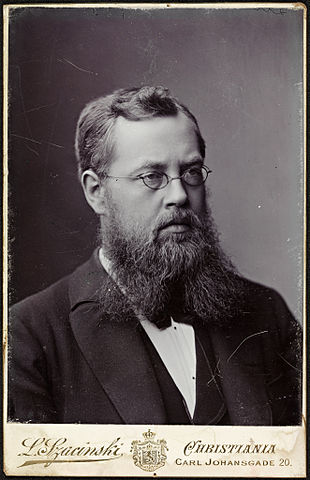
\includegraphics[width=10em]{assets/img/sophus_lie.jpg}
\caption*{Portrait of Marius Sophus Lie}
\end{figure}

Marius Sophus Lie was a Norwegian-born mathematician.
He created the theory of \textbf{continuous symmetry}, and applied it to
the study of geometry and differential equations. Among his greatest
achievements was the discovery that continuous transformation
groups are better understood in their linearized versions
(``Theory of transformation groups'' 1893).
These \textbf{infinitesimal generators} form a structure which is today
known as a \textbf{Lie algebra}. The linearized version of the group law
corresponds to an operation on the Lie algebra known as
the \textbf{commutator bracket} or \textbf{Lie bracket}.
1882 Professor in Christiania (Oslo),
1886 Leipzig (succeeding Felix Klein),
1898 Christiania.


\subsubsection{The Exponential Map}%
\label{ssub:the_exponential_map}

Given the infinitesimal formulation of rotation,
we got to the differential equation system:
	\[\left\{ \begin{aligned}
		\dot{R}(t) &= \widehat{w}(t)R(t) \\
		R(0) &= I \\
	\end{aligned}\right.\]

If we assume that $\widehat{w}(t)$ is constant in time ($=\widehat{w}$),
this known equation has the solution:
	\[R(t) = e^{\widehat{w}t}
		= \sum_{n=0}^{\infty} \frac{{(\widehat{w}t)}^n }{n!}
		= I + \widehat{w}t + \frac{{(\widehat{w}t)}^2 }{2!} + \ldots \]

which is a rotation around the axis $w \in \R^3$
by an angle of t (if $\|w\| = 1$). Alternatively, one can absorb
the scalar $t \in \R$ into the skew  symmetric matrix $\widehat{w}$
to obtain $R(t) = e^{\widehat{v}}$ with $\widehat{v} = \widehat{w}t$.
This \textbf{matrix exponential} therefore defines a map from
the Lie algebra to the Lie group:
	\[\exp : so(3) \rightarrow SO(3);\quad \widehat{w}\mapsto e^{\widehat{w}}\]


\subsubsection{The Logarithm of $SO(3)$}%
\label{ssub:the_logarithm_of_so_3_}

There is conversely a mapping from the Lie group to the Lie algebra.
For any rotation matrix $R \in SO(3)$, there exists a $w \in \R^3$
such that $R = \exp(\widehat{w})$. Such an element is denoted by
$\widehat{w} = \log(R)$. If $R \ne I$, we note $r_{ij}$ its coefficients
and $w$ is given by:
	\[\left\{ \begin{aligned}
		|w| &= \inv{\cos}\left(\frac{\text{trace}(R)-1}{2}\right)\\
		\frac{w}{|w|} &= \frac{1}{2\sin(|w|)}
			\begin{pmatrix}
				r_{32} - r_{23} \\
				r_{13} - r_{31} \\
				r_{21} - r_{12} \\
			\end{pmatrix}
	\end{aligned}\right.\]

For $R = I$, we have $|w| = 0$, i.e.\ a rotation by an angle 0.
The above statement says:
\textbf{Any orthogonal transformation $\bm{\R \in SO(3)}$ can be realized
by rotating by an angle $\bm{|w|}$ around an axis
$\bm{\frac{w}{|w|}}$ as defined above}.\\

Obviously the above representation is not unique since for example,
increasing the angle by multiples of $2\pi$ will give the same rotation.


\subsubsection{Rodrigues' Formula}%
\label{ssub:rodrigues_formula}

In analogy to the well-known Euler equation
	\[\forall \phi \in \R, \quad  e^{i\phi} = \cos(\phi) + i\ \sin(\phi)\]

we have an expression for skew symmetric matrices $\widehat{w} \in so(3)$:
	\[\boxed{
	e^{\widehat{w}} = I + \frac{\widehat{w}}{|w|} \sin(|w|)
		+ \frac{\widehat{w}^2}{|w|^2} (1 - \cos(|w|))}\]

This is known as \textbf{Rodrigues' formula}.\\

\underline{Proof sketch:}
Let $t = |w|$ and $v = w/|w|$ such that $w = vt$. Then one can show that:
	\[\widehat{v}^2 = v\tr{v} - I \quad
	\text{and}\quad \widehat{v}^3 = -\widehat{v}\]
Thus, by developing the exponential, we get:
	\[e^{\widehat{v}t} = I +
		\underbrace{\left( t - \frac{t^3}{3!} + \cdots \right)}_{\sin(t)}\widehat{v}
	+ \underbrace{\left(\frac{t^2}{2!}-\frac{t^4}{4!}+\cdots \right)}_{1-\cos(t)}
		\widehat{v}^2\]


\subsection{The Lie Group $SE(3)$}%
\label{sub:the_lie_group_se_3_}


\subsubsection{Representation of Rigid-body Motions $SE(3)$}%
\label{ssub:representation_of_rigid_body_motions_se_3_}

We have seen that the space of rigid-body motions is given by
the group of special Euclidean transformations:
	\[SE(3) \equiv \{ g = (R,T)\ |\ R \in SO(3),\ T \in \R^3\}\]
In homogeneous coordinates:
	\[\boxed{SE(3) \equiv
	\left\{ g = \begin{pmatrix}
		R & T \\
		0 & 1 \\
	\end{pmatrix}\ \middle|\ R \in SO(3), T \in \R^3\right\}}\]

In the context of rigid motions, one can see the difference
between points in $\E^3$ (which can be rotated and translated)
and vectors in $\R^3$ (which can only be rotated).


\subsubsection{The Lie Algebra of Twists}%
\label{ssub:the_lie_algebra_of_twists}

Given a continuous family of rigid-body transformations:
	\[g : \R \rightarrow SE(3);\quad g(t) = \begin{pmatrix}
		R(t) & T(t) \\
		0 & 1 \\
	\end{pmatrix}\ \in \RR{4}{4}\]

we consider:
	\[\dot{g}(t)\inv{g}(t) = \begin{pmatrix}
		\dot{R}\tr{R} & \dot{T} - \dot{R}\tr{R}T \\
		0 & 0 \\
	\end{pmatrix}\ \in \RR{4}{4}\]

As in the case of $SO(3)$ the $\dot{R}\tr{R}$ corresponds
to some skew-symmetric matrix $\widehat{w} \in so(3)$. Defining a vector
$v(t) = \dot{T}(t) - \widehat{w}(t)T(t)$, we have:
	\[\dot{g}(t)\inv{g}(t) = \begin{pmatrix}
		\widehat{w}(t) & v(t) \\
		0 & 0 \\
	\end{pmatrix} \equiv \widehat{\xi}(t) \in \RR{4}{4}\]

Multiplying with $g(t)$ from the right, we obtain:
	\[\dot{g} = \dot{g}\inv{g}g = \widehat{\xi}g\]

The $4 \times 4$ matrix $\widehat{\xi}$ can be viewed as a tangent vector
along the curve $g(t)$. $\widehat{\xi}$ is called a \textbf{twist}.
As in the case of $so(3)$, the set of all twists forms the tangent
space which is the \textbf{Lie algebra}
	\[\boxed{se(3) \equiv \left\{ \widehat{\xi} = \begin{pmatrix}
		\widehat{w} & v \\
		0 & 0 \\
	\end{pmatrix}\ \middle|
	\ \widehat{w} \in so(3),\ v \in \R^3 \right\}}\]

	to the \textbf{Lie group $\bm{SE(3)}$}.\\

As before, we can define operators $\wedge$ and $\vee$ to convert between
a \textbf{twist $\bm{\widehat{\xi} \in se(3)}$} and its
\textbf{twist coordinates} $\bm{ \xi \in \R^6 }$:
	\[\widehat{\xi} \equiv \begin{pmatrix} v \\ w \end{pmatrix}^{\wedge}
		\equiv \begin{pmatrix}
			\widehat{w} & v \\
			0 & 0
		\end{pmatrix}\ \in \RR{4}{4}\]

	\[\begin{pmatrix}
		\widehat{w} & v \\
		0 & 0
	\end{pmatrix}^{\vee} \equiv \begin{pmatrix} v \\ w \end{pmatrix} \in \R^6\]


\subsubsection{Exponential Coordinates for $SE(3)$}%
\label{ssub:exponential_coordinates_for_se_3_}

The twist coordinates $\xi = \inmatrix{v\\w}$ are formed by stacking the
\textbf{linear velocity} $\bm{v \in \R^3}$ (related to translation) and the
\textbf{angular velocity} $\bm{w \in \R^3}$ (related to rotation).\\

The differential equation system:
	\[\left\{ \begin{aligned}
		\dot{g}(t) &= \widehat{\xi}g(t), \quad \widehat{\xi} = \text{const}\\
		g(0) &= I
	\end{aligned} \right.\]

has the solution $g(t) = e^{\widehat{\xi}t} = \sum_{n=0}^{\infty}
\frac{{(\widehat{\xi}t)}^n}{n!}$.
For $w = 0$, we have $e^{\widehat{\xi}} = \inmatrix{I & v \\ 0 & 1}$,
while for $w \ne 0$ one can show:
	\[\boxed{e^{\widehat{\xi}} = \begin{pmatrix}
		e^{\widehat{w}} & \frac{(I-e^{\widehat{w}})\widehat{w}v + w\tr{w}v}{|w|^2}\\
		0 & 1
	\end{pmatrix}}\]

The above shows that the exponential map defines a transformation from
the Lie algebra $se(3)$ to the Lie group $SE(3)$:
	\[ \exp:\ se(3) \rightarrow SE(3);\ \widehat{\xi} \mapsto e^{\widehat{\xi}}\]

The elements $\widehat{\xi} \in se(3)$ are called the
\textbf{exponential coordinates} for $SE(3)$.\\

\underline{Conversely:} \textbf{For every $\bm{g \in SE(3)}$ there exist
twist coordinates $\bm{\xi = (v,w) \in \R^6}$ such that $\bm{g=\exp(\widehat{\xi})}$.}\\

\underline{Proof sketch:} Given $g = (R,T)$, we merely need to solve the equation
for the velocity vector $v \in \R^3$:
	\[\frac{(I-e^{\widehat{w}})\widehat{w}v + w\tr{w}v}{|w|^2} = T\]


Be aware that, just as in $SO(3)$, \textbf{this representation is not unique}.
In general, there exist many twists representing the same rigid-body motion.


\subsection{Representing the Camera Motion}%
\label{sub:representing_the_camera_motion}

When observing a scene from a moving camera, the coordinates and velocity
of points in camera coordinates will change. We will use a rigid-body transformation
	\[g(t) = \begin{pmatrix}
		R(t) & T(t) \\
		0 & 1
	\end{pmatrix}\ \in SE(3)\]

to represent the motion from a fixed world frame to the camera frame at time $t$.
In particular, we assume that at time $t=0$ the camera frame coincides with the
world frame, i.e.\ $g(0)=I$.
For any point $\bm{X_0}$ in world coordinates,
its coordinates in the camera at time $t$ are:
	\[\bm{X}(t) = R(t)\bm{X_0} + T(t)\]

or in the homogeneous representation:
	\[\bm{X}(t) = g(t)\bm{X_0}\]

Please remark that for practicity, we use the same notation
in 3D coordinates and homogeneous coordinates but these are different.


\subsubsection{Concatenation of Motions over Frames}%
\label{ssub:concatenation_of_motions_over_frames}

Given two different times $t_1$ and $t_2$, we denote the transformation from
the points in frame $t_1$ to the points in frame $t_2$ by $g(t_2,t_1)$:
	\[\bm{X}(t_2) = g(t_2,t_1) \bm{X}(t_1)\]

Those transformations composes, and we can very easily show that:
	\[g(t_3,t_1) = g(t_3,t_2) g(t_2,t_1)\]

and
	\[\inv{g}(t_2,t_1) = g(t_1,t_2)\]


\subsubsection{Rules of Velocity Transformation}%
\label{ssub:rules_of_velocity_transformation}

Since the coordinates of point $\bm{X}_0$ in frame $t$ are given by
$\bm{X}(t) = g(t) \bm{X}_0$, the velocity is given by:
	\[\bm{\dot{X}}(t) = \dot{g}(t)\bm{X}_0 = \dot{g}(t)\inv{g}(t) \bm{X}(t)\]

By introducing the \textbf{twist coordinates}:
	\[\widehat{V}(t) \equiv \dot{g}(t)\inv{g}(t) = \begin{pmatrix}
		\widehat{w}(t) & v(t) \\
		0 & 0 \\
	\end{pmatrix}\ \in se(3)\]

we get the expression:
	\[\boxed{\bm{\dot{X}}(t) = \widehat{V}(t)\bm{X}(t)}\]

which in simple 3D-coordinates gives:
	\[\bm{\dot{X}}(t) = \widehat{w}(t)\bm{X}(t) + v(t)\]


\subsubsection{Transfer Between Frames: The Adjoint Map}%
\label{ssub:transfer_between_frames_the_adjoint_map}

Suppose that a viewer in another frame A is displaced relative to the current frame
by a transformation $g_{xy}$: $\mathbf{Y}(t) = g_{xy} \mathbf{X}(t)$.
Then the velocity in this new frame is given by:
\[\mathbf{\dot{Y}}(t)
	= g_{xy} \mathbf{\dot{X}}(t)
	= g_{xy} \widehat{V}(t) \mathbf{X}(t)
	= g_{xy} \widehat{V} \inv{g_{xy}} \mathbf{Y}(t)\]

This shows that the relative velocity of points observed from camera frame A
is represented by the twist
\[\widehat{V}_y = g_{xy} \widehat{V} \inv{g_{xy}}
	\equiv \text{ad}_{g_{xy}}(\widehat{V})\]

where we have introduced the \textbf{adjoint map on $se(3)$}:
\[\text{ad}_g : se(3) \rightarrow se(3);
	\widehat{\xi} \mapsto g \widehat{\xi} \inv{g}\]


\subsection{Summary of Lie Transformations}%
\label{sub:summary_of_lie_transformations}


\begin{table}[ht]
\centering
\begin{tabular}{rcc}
& Rotation $SO(3)$ & Rigid-body $SE(3)$ \\ \midrule
	Matrix representation
	& \makecell{$R \in GL(3)$ \\ $\tr{R}R = I$ \\ $\det(R) = 1$}
		% & $g = \inmatrix{R & T \\ 0 & 1}$
		& $g = \begin{pmatrix}R & T \\ 0 & 1\end{pmatrix}$
		\\
	3-D coordinates
		& $\mathbf{X} = R \mathbf{X}_0$
		& $\mathbf{X} = R \mathbf{X}_0 + T$
		\\
	Inverse
		& $\inv{R} = \tr{R}$
		& $\inv{g} = \inmatrix{\tr{R} & -\tr{R}T \\ 0 & 1}$
		\\
	Exp representation
		& $R = \exp{\widehat{w}}$
		& $g = \exp{\widehat{\xi}}$
		\\
	Velocity
		& $\mathbf{\dot{X}} = \widehat{w} \mathbf{X}$
		& $\mathbf{\dot{X}} = \widehat{w} \mathbf{X} + v$
		\\
	Adjoint map
		& $\widehat{w} \mapsto R \widehat{w} \tr{R}$
		& $\widehat{\xi} \mapsto g \widehat{\xi} \inv{g}$
		\\
\end{tabular}
\caption{Summary of Lie Transformations}%
\label{tab:summary_lie_transformations}
\end{table}


\section{Visual Odometry}%
\label{sec:visual-odometry}

\subsection{Direct VS Indirect}%
\label{sub:direct-indirect}

\subsubsection{Feature Points}%
\label{ssub:feature-points}

\subsubsection{Direct Formulation}%
\label{ssub:direct-formulation}

\begin{figure}[ht]
	\centering
	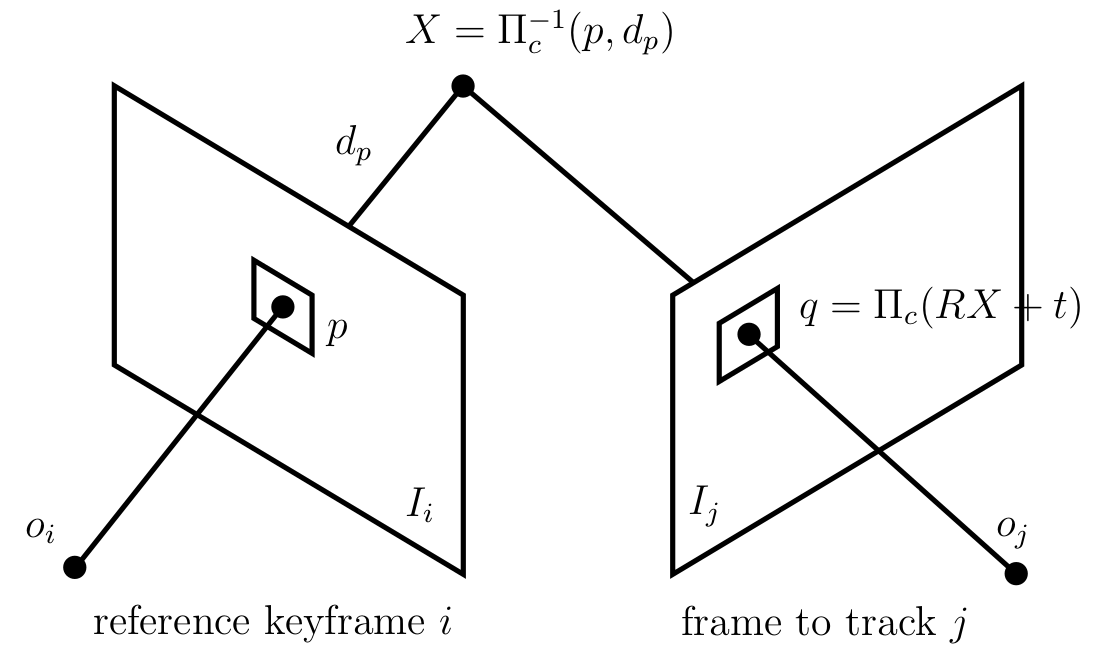
\includegraphics[width=\linewidth]{assets/img/direct-image-alignment.png}
	\caption{Direct image alignment}%
	\label{fig:direct-image-alignment}
\end{figure}

\begin{figure}[ht]
	\centering
	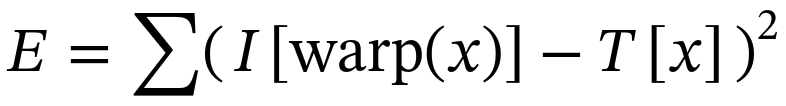
\includegraphics[width=\linewidth]{assets/img/energy-warp.png}
	\caption{Energy formulation for direct image alignment}%
	\label{fig:energy-warp}
\end{figure}

\begin{figure}[ht]
	\centering
	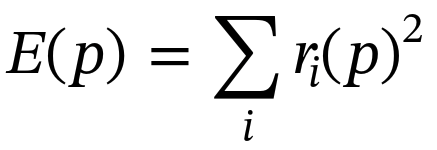
\includegraphics[width=\linewidth]{assets/img/energy-gauss-newton.png}
	\caption{Energy formulation for Gauss-Newton minimization}%
	\label{fig:energy-gauss-newton}
\end{figure}

\begin{figure}[ht]
	\centering
	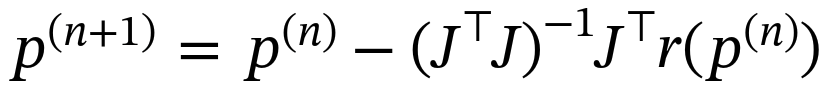
\includegraphics[width=\linewidth]{assets/img/gauss-newton-step.png}
	\caption{Gauss-Newton step}%
	\label{fig:gauss-newton-step}
\end{figure}

\subsection{RGB-D Visual Odometry}%
\label{sub:rgbd-visual-odometry}

\begin{figure}[ht]
	\centering
	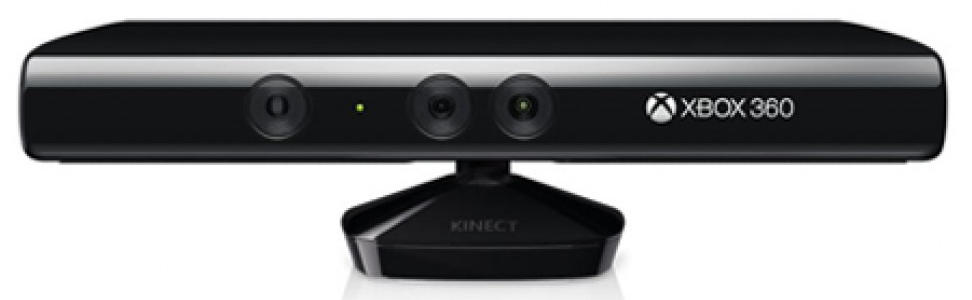
\includegraphics[width=\linewidth]{assets/img/kinect.jpg}
	\caption{Kinect sensor}%
	\label{fig:kinect}
\end{figure}

\section{Visual SLAM}%
\label{sec:v-slam}

\begin{figure}[ht]
	\centering
	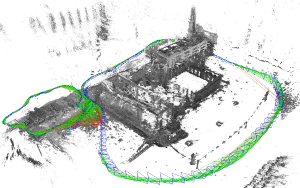
\includegraphics[width=\linewidth]{assets/img/lsd-slam.png}
	\caption{LSD-SLAM}%
	\label{fig:lsd-slam}
\end{figure}

\subsection{Pose Graph}%
\label{sub:pose-graph}

\begin{figure}[ht]
	\centering
	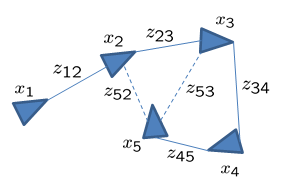
\includegraphics[width=\linewidth]{assets/img/pose-graph.png}
	\caption{Pose graph}%
	\label{fig:pose-graph}
\end{figure}

\subsection{Loop Closure}%
\label{sub:loop-closure}

\begin{figure}[ht]
	\centering
	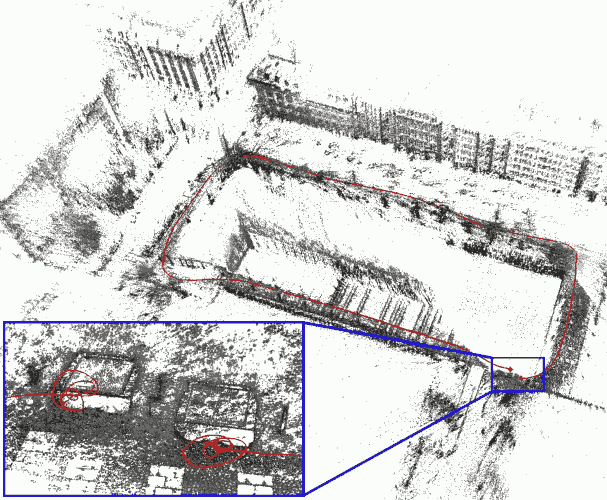
\includegraphics[width=\linewidth]{assets/img/loop-closure-lowres.png}
	\caption{Loop closure}%
	\label{fig:loop-closure}
\end{figure}
